%Max 1500w or 4 pages
%Deadline 17:00 on Tuesday 09-02-2016

\section{Introduction}

The project aims to create a micro-modelled road traffic simulation engine enabling inspection of various effects of changing key rules within the model. For team members, this project is centered around teamwork and also, as a less prominent addition, the learning and application of software engineering skills within a group setting.

\section{Project Description} %~60% of the report
%Describe your team’s aims for the projects. Outline what aims your team have set for the project and your strategy for achieving those aims. A rough timetable may be appropriate and you may wish to break your aims into levels (e.g. mandatory / optional or we will first work on level 1 aims before moving to level 2 aims) to allow for unexpected issues that may arise. You must also describe how your initial progress developing your piece of software has gone and where you currently are relative to your aims.

\subsection{Simulation Model}
The project started with a research phase to determine the general approaches to micro and macro models in order to decide which one the team would use for the simulation. After a vote the micro model was unanimously chosen for its precise granular control over the agents down to the individual ones within the simulation.

\vspace{2mm}

As the micro-model implementation focuses on individual representation of cars as physical objects and individual tuning of their parameters the starting point chosen is based on the Nagel–Schreckenberg model. The roads in this model are represented as cellular automata\cite{Schreckenberg}. In this, each cell can either be occupied by an object or be empty. Cars can have different properties such as acceleration, speed, direction and can move to other free neighbouring cells. The model can be expanded through the use of graphs to connect roads.

\vspace{2mm}

In the early stages streets will be arranged to model simple road networks and, in later ones, more realistic ones.
Rules in the simulation will include driving rules such as crossings, lane changes, etc.., and laws of physics. That can be further expanded to include weather factors and engine emissions for example.

\vspace{2mm}

The simulation system will be used to gather relevant data on the reaction of the model to changing rules for analysis. This will include road network throughput and congestion effects.

\subsection{Architecture}

A brainstorming session hewed a rough architectural outlay of the product. It breaks down into three main artefacts:
\vspace{1mm}
\begin{itemize}
	\item the GUI,
	\item the simulation engine and
	\item a log library module.
\end{itemize}
\vspace{1mm}
The simulation engine will be broken up into smaller pieces as it is not only the centrepiece of the project but also the biggest part (see Figure~\ref{fig:arch_overview}).

\begin{figure}[h!]
	\vspace{1.5em}
  	\caption{Rough architecture overview}
  	\label{fig:arch_overview}
  	\centering
	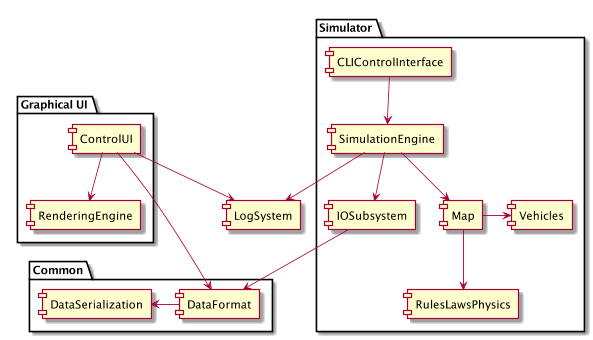
\includegraphics[width=0.5\textwidth]{figs/arch_diagram.png}
  	\vspace{1.5em}
\end{figure}

\subsection{Development}

Once a rough architecture and the tooling is set-up the plan is to start developing modules as early as possible to get a basic system working before reaching the 2\textsuperscript{nd} milestone so as to have a buffer in the event of unforeseen setbacks.

\vspace{2mm}

Java was chosen as the development language as all members of the team have, at the very least, some familiarity with it. It also is cross-platform, has GUI capabilities and has a slew of libraries and tools available for it.

\subsection{Preliminary Timetable \& Current project status}

The timetable is broken into 4 major milestones and each of those encompass a set of goals to be completed by the date (see Table~\ref{tab:milstones}).

\vspace{2mm}

\begin{table}[h]
	\vspace{1.5em}
	\caption{Preliminary Milestones descriptions and current statuses}
	\label{tab:milstones}
	\centering
	\resizebox{\linewidth}{!}{%
\begin{tabular}{lc}
\rowcolor[HTML]{656565}
{\color[HTML]{FFFFFF} \textbf{Milestone timetable}} & {\color[HTML]{FFFFFF} \textbf{Status}} 					\\ \hline
\multicolumn{2}{l}{\textbf{9th Feb - Milestone I: Preliminary report submission}}       						\\ \hline
Team structure ready           																					& \checkmark \\
Team process setup (communication, teamwork, knowledge sharing, visibility)         							& \checkmark \\
Graple deployment harness																						& \checkmark \\
Basic log system																								& \checkmark \\
Rough architecture outlined, some basics set for modelling		                    							& \checkmark \\ \hline
\multicolumn{2}{l}{\textbf{1st Mar - Milestone II: Basic Functionalities implemented and working}}   			\\ \hline
Basic modelling ready: simple roads with different physical object properties									& \\
Basic tooling support: setting up testbed parameters, map, parameters of active objects 			       		& \\
Full multi-output (terminal, txt file and csv file) functionalities in Log system completed						& \\
Basic measurements ready: log output, throughput measurements, simulation saving								& \\
Basic GUI ready: display animations either from live simulation or saved as a file 								& \\ \hline
\multicolumn{2}{l}{\textbf{25th Mar - Milestone III: Possible advanced functionalities implemented and working}}\\ \hline
Optional: Larger size of the model: graph with many connections                									& \\
Optional: Loading map data from actual OpenStreetMap sources (filtering highways, counting lanes, etc...) 		& \\
Optional: Attempting in-model traffic lights and model parameters optimization with different algorithms        & \\ \hline
\multicolumn{2}{l}{\textbf{31st Mar - Milestone IV: Final report submission}}		\\ \hline
Code prepared and ensured for correctness and visibility 														& \\
Report ready and submitted. 																					& \\
Presentation ready \& rehearsed 																				& \\ \hline
\end{tabular}}
	\vspace{1.5em}
\end{table}

As the table describes, the team has already completed all the set-ups of processes to facilitate development and communication, and has also started coding the log module necessary to facilitate hunting down any issues in the code when run when they arise. Essentially, the 1\textsuperscript{st} milestone's tasks have been completed ahead of time.

\section{Project Organisation} %~40% of the report
The project is organized around the skills team members have, and tools which can be used to achieve best results. The main
principles are flat team organization (no management relations), peer interaction (reviews, help) and an overall agile
approach development. The concept of project advancement is built on the notion of Minimal Viable Product and
iterative improvements with team-wide backlog prioritization.

Each team member bears equal rights and responsibilities and, in addition to that, the project coordinator has the extra responsibility
of ensuring that the artefacts are delivered on time. Peer assessment is set as equal participation/equal assessment.

\subsection{Process and Teamwork}
\subsubsection{Cooperation}
%This is probably already covered in section 1 - the task%
The development process approach is revolving around main aims of the project - that being not only building the product
satisfying specification, but also learning form each other and attempting the agile and responsible teamwork model.

Tasks are distributed according to module choice and skills. Existing team member experience is used to the most
possible extent.

As soon as there are multiple opinions on any decision to be made, following procedure should be applied:

\begin{enumerate}
    \item Two conflicting parties try to persuade each other using logic
    \item In case consensus not found, all the team is involved to the mutual persuasion
    \item In case consensus not yet found, voting is attempted (public, majority rule). Team size of 5 guarantees decision.
        Everyone should follow this decision even if they were opposing party.
\end{enumerate}

As each team member is anticipated to invests similar effort into the project, votes are always equal.

\subsubsection{Meetings}
In addition to ad-hoc meetings there is a planned weekly iterated meeting on Tuesdays. Meeting agenda is created in advance and everyone can
contribute. Meeting minutes are added as comments to the appropriate Trello\footnote{Trello is an agile process and information organisation tool having card and board notion, moving the concept of sticky notes and board to software world https://trello.com/tour} card.

\subsubsection{Development Process}

The team has decided to follow a simplistic Kanban-like\cite{Ahmed} agile development process, with individual work items piled into backlog,
which is then prioritised by all team members. Team members pick up the tasks from the top of the stack which match their skill set
and module specialisation. The team will adopt new techniques and elements of the process as project course demands.
The same agile continuous refinement and improvement process is applied to the architecture.

\vspace{2mm}

The selected process is development-centric, it defines rules of how features are specified, implemented, tested and eventually
merged into the main git repository, and how visibility is achieved. The card system allows for clear classification of an activity by specific team member, component, status, priority, and activity progress. Commenting is then used for information exchange on that specific activity. Activities can be features, bugs, non-code items, research items, etc. The board as a whole gives snapshot of the current project status, and also provides full change history.

\vspace{2mm}

Unit testing has a dedicated place within the process. Every commit should be accompanied by appropriate unit tests, and code should have
inline documentation supplied. Obligatory post-commit peer code review aims at improving code quality as well as ensuring the rules are abided.

\subsubsection{Tools}

Due to the distributed and asynchronous project nature, software tools play an important role in ensuring the overall success. Following are descriptions of \emph{development tools} chosen for the project:

\vspace{1mm}

\begin{itemize}
	\item Git and GitHub. Git is used as a primary code exchange point, communication tool by using appropriate commit messages. Frequent updates are an important project practice. At the time of writing this report, team does not yet utilize forked feature branches and pull requests approach. It is anticipated that team will switch to this approach after delivery of Minimal Viable Product. \\GitHub is a primary tool for code review, as it allows for post-commit code commenting.
	\item Build System to ensure build portability and easy project model exchange.
	 Gradle\footnote{Gradle is a task-based sophisticated build automation tool for Java and more. http://gradle.org} has been chosen as a build tool for the project, since it allows for easy plugin architecture, is quick and easy to setup. %and IntelliJ IDEA has great Gradle integration features.
	 Gradle is used to automate routine jobs of build, test, assembly  and documentation generation,
	as well as provide more in-depths analysis tools such as providing test coverage metrics.\\Gradle wrapper is also committed to the main code repository, so the build is configuration-agnostic and requires only the JDK only in a minimal setup.
	\item IntelliJ IDEA\footnote{We decided to use IntelliJ IDEA Community Edition, https://www.jetbrains.com/idea/download/}. Selected as an IDE of choice as it may greatly improve productivity and has means for extensive refactoring functionality. IDEA has an outstanding
	integration with Gradle builds, allowing to run the build tasks from within itself.
	\item Unit Testing. jUnit 4, Mockito and Fest-assert\footnote{Following article has been used as a base for testing environment setup http://blog.codeleak.pl/2013/07/test-code-readability-improved-junit.html} libraries are used to provide reliable and regression-resistant code base. Unit testing is one of the key development activities within the project's scope.
\end{itemize}

\vspace{1mm}

In addition to development tools, the following communication and documentation tools are of absolute importance for the project to succeed:

\vspace{1mm}

\begin{itemize}
	\item Trello is a web and mobile based collaboration tool that organises projects into boards. With this distinctive feature, it is simple to use. Trello can be used as a Kanban board with tasks represented with cards facilitating the viewing of the current progress status of the project. In addition to storing tasks as cards on the board, cards can also be used for easy information storage and exchange, forming essentially a loosely coupled knowledge base of links, ideas and preliminary research results which can be called upon by any team member.
	\item HipChat\footnote{Atlassian web chat product, based on open Jabber protocol, https://www.hipchat.com} is used as the primary communication tool. Being a webchat with separate rooms and offering web, mobile and desktop clients, it offers a myriad of different integrations. For now, only the GitHub and Trello integrations are used. Both post their activities/updates to the IM (commits, pulls, etc... for GitHub and edits, comments, etc... for Trello).
	\item PlantUML for diagrams. Since PlantUML allows to create diagrams using text files, they are extremely easy to version alongside the main code in the source control. Non-WYSIWYG editors for diagram also have the added bonus of saving time on object arrangement, forcing user to spend more time on semantics rather than positioning.
	\item LaTeX is used for generating the preliminary and final project reports.
\end{itemize}